\let\lesson\undefined
\newcommand{\lesson}{\phantomlesson{Bài 17: Động năng và thế năng. Định luật bảo toàn cơ năng.}}
\chapter[Định luật bảo toàn cơ năng.]{Định luật bảo toàn cơ năng.}
\setcounter{section}{0}
\section{Lý thuyết}
\subsection{Cơ năng của một vật chuyển động trong trọng trường}
Khi một vật chuyển động trong trọng trường thì tổng động năng và thế năng của vật được gọi là cơ năng của vật trong trọng trường (gọi tắt là cơ năng của vật).

Kí hiệu cơ năng của vật là $W$:
\begin{equation*}
	W=W_\text{đ}+W_\text{t}=\dfrac{1}{2}mv^2+mgz\label{CT-conang},
\end{equation*}
trong đó:
\begin{itemize}
	\item $W$ là cơ năng của vật;
	\item $W_\text{đ}=\dfrac{1}{2}mv^2$ là động năng của vật;
	\item $W_\text{t}=mgz$ là thế năng của vật.
\end{itemize}

\subsection{Bảo toàn cơ năng của vật chuyển động trong trọng trường}
Khi một vật chuyển động trong trọng trường chỉ chịu tác dụng của trọng lực thì cơ năng của vật là một đại lượng bảo toàn.
\begin{equation*}
	W=W_\text{đ}+W_\text{t}=\dfrac{1}{2}mv^2+mgz=\textrm{hằng số}
\end{equation*}

\textit{Hệ quả:}
\begin{itemize}
	\item Nếu động năng giảm thì thế năng tăng (động năng chuyển hóa thành thế năng) và ngược lại.
	\item Tại vị trí nào động năng cực đại thì thế năng cực tiểu và ngược lại.
\end{itemize}
\ppgiai{
	\begin{description}
		\item[Bước 1:] Chọn mốc thế năng. Viết biểu thức cơ năng cho vị trí lúc đầu và lúc sau.
		
		Cơ năng cho vị trí lúc đầu, ta gọi là vị trí 1:
		\begin{equation*}
			W_1=W_\text{đ1}+W_\text{t1}=\dfrac{1}{2}mv_1^2+mgz_1.
		\end{equation*}
		
		Cơ năng cho vị trí lúc sau, ta gọi là vị trí 2:
		\begin{equation*}
			W_2=W_\text{đ2}+W_\text{t2}=\dfrac{1}{2}mv_2^2+mgz_2.
		\end{equation*}
		
		\item[Bước 2:] Áp dụng định luật bảo toàn cơ năng
		\begin{eqnarray*}
			W_1&=&W_2\\
			\Rightarrow W_\text{đ1}+W_\text{t1} &=& W_\text{đ2}+W_\text{t2}\\
			\Rightarrow \dfrac{1}{2}mv_1^2+mgz_1 &=& \dfrac{1}{2}mv_2^2+mgz_2.
		\end{eqnarray*}
	\end{description}
}
\subsection{Biến thiên cơ năng của vật chuyển động trong trọng trường}
Khi một vật chuyển động trong trọng trường, nếu vật chịu tác dụng thêm lực cản (không phải lực thế) thì cơ năng của vật sẽ biến đổi. Công của lực cản bằng độ biến thiên của cơ năng.
\begin{equation*}
	A=W_2-W_1,
\end{equation*}
trong đó:
\begin{itemize}
	\item $A$ là công của lực cản;
	\item $W_1$ là cơ năng lúc đầu ở vị trí 1;
	\item $W_2$ là cơ năng lúc sau ở vị trí 2.
\end{itemize}

\ppgiai{
	\begin{description}
		\item[Bước 1:] Chọn mốc thế năng. Viết biểu thức cơ năng cho vị trí lúc đầu và lúc sau.
		
		Cơ năng cho vị trí lúc đầu, ta gọi là vị trí 1:
		\begin{equation*}
			W_1=W_\text{đ1}+W_\text{t1}=\dfrac{1}{2}mv_1^2+mgz_1.
		\end{equation*}
		
		Cơ năng cho vị trí lúc sau, ta gọi là vị trí 2:
		\begin{equation*}
			W_2=W_\text{đ2}+W_\text{t2}=\dfrac{1}{2}mv_2^2+mgz_2.
		\end{equation*}
		
		\item[Bước 2:] Viết biểu thức tính công của lực cản (không phải lực thế) bằng độ biến thiên của cơ năng.
		\begin{equation*}
			A=W_2-W_1=\left(\dfrac{1}{2}mv_2^2+mgz_2\right)-\left(\dfrac{1}{2}mv_1^2+mgz_1\right).
		\end{equation*}
	\end{description}
}

\section{Mục tiêu bài học - Ví dụ minh họa}
\begin{dang}{Biện luận sự chuyển hóa giữa động năng và thế năng}
	
	\viduii{2}{
		Một vật có khối lượng $m=\SI{1}{kg}$ được thả rơi tự do từ độ cao $\SI{20}{m}$ so với mặt đất. Chọn gốc thế năng tại mặt đất. Bỏ qua mọi ma sát. Ngay khi vật chạm đất thì
		\begin{mcq}
			\item động năng cực đại, thế năng cực tiểu.
			\item động năng bằng thế năng.
			\item động năng cực tiểu, thế năng cực đại.
			\item động năng bằng một nửa thế năng.
		\end{mcq}
	}
	{\begin{center}
			\textbf{Hướng dẫn giải}
		\end{center}
		
		Trong quá trình rơi, vận tốc của vật tăng dần còn độ cao giảm dần. Do đó, khi vật chạm đất thì vận tốc lớn nhất nên động năng cực đại, còn độ cao nhỏ nhất nên thế năng cực tiểu.
		
		\textbf{Đáp án: A}.
		
	}
	\viduii{2}{
		Một vật có khối lượng $m=\SI{1}{kg}$ được ném lên với vận tốc $\SI{10}{m/s}$ từ độ cao $\SI{1}{m}$ so với mặt đất. Chọn gốc thế năng tại mặt đất. Bỏ qua mọi ma sát. Ngay khi vật lên đến độ cao cực đại thì
		\begin{mcq}
			\item động năng cực đại, thế năng cực tiểu.
			\item động năng bằng thế năng.
			\item động năng cực tiểu, thế năng cực đại.
			\item động năng bằng một nửa thế năng.
		\end{mcq}
	}
	{\begin{center}
			\textbf{Hướng dẫn giải}
		\end{center}
		
		Trong quá trình vật bay lên, vận tốc giảm dần còn độ cao tăng dần. Do đó, khi vật lên đến độ cao cực đại thì thế năng cực đại vì độ cao cực đại, còn động năng cực tiểu vì vận tốc cực tiểu.
		
		\textbf{Đáp án: C}.
	}
\end{dang}
\begin{dang}{Xác định cơ năng của vật chuyển động trong trọng trường}
	\viduii{2}{Một vật có khối lượng $\SI{2}{kg}$ rơi tự do không vận tốc đầu từ độ cao $\SI{5}{m}$ xuống mặt đất. Nếu chọn gốc thế năng tại mặt đất, lấy $g=\SI{10}{m/s^2}$, cơ năng của vật có giá trị 
		\begin{mcq}(4)
			\item $\SI{10}{J}$.
			\item $\SI{100}{J}$.
			\item $\SI{50}{J}$.
			\item $\SI{5}{J}$.
		\end{mcq}
	}
	{	\begin{center}
			\textbf{Hướng dẫn giải}
		\end{center}
		Cơ năng của vật bằng tổng động năng và thế năng. Tại thời điểm bắt đầu rơi, vận tốc của vật bằng không, giá trị cơ năng tương ứng là 
		\begin{align*}
			W&=W_\text{đ}+W_\text{t}\\
			&=\dfrac{1}{2}mv^2+mgh\\
			&=\dfrac{1}{2}\cdot\SI{2}{\kilogram}\cdot(\SI{0}{\meter/\second})^2+\SI{2}{\kilogram}\cdot\SI{10}{\meter/\second^2}\cdot\SI{5}{\meter}\\
			&=\SI{100}{\joule}.
		\end{align*}
		
		\textbf{Đáp án: B.}
		
		\begin{center}
			\textbf{Câu hỏi tương tự}
		\end{center}
		
		Từ điểm M (có độ cao so với mặt đất bằng $\SI{0,8}{\meter}$) ném lên một vật với vận tốc đầu $\SI{2}{\meter/\second}$. Biết khối lượng của vật bằng $\SI{0,5}{\kilogram}$, lấy $g=\SI{10}{\meter/\second^2}$. Chọn mốc thế năng tại mặt đất, cơ năng của vật bằng bao nhiêu?
		
		\textbf{Đáp án:} $\SI{5}{\joule}$.
	}
	\viduii{3}{Một vật có khối lượng $\SI{100}{\gram}$ được ném thẳng đứng từ độ cao $\SI{5}{\meter}$ lên phía trên với vận tốc đầu là $\SI{10}{\meter/\second}$. Bỏ qua lực cản của không khí. Lấy $g=\SI{10}{\meter/\second^2}$. Xác định cơ năng của vật ở thời điểm $\SI{0,5}{\second}$ kể từ khi chuyển động.
	}
	{	\begin{center}
			\textbf{Hướng dẫn giải}
		\end{center}
		
		Chọn mặt đất là mốc thế năng, chiều dương là chiều từ mặt đất lên cao. Trường hợp này vật chuyển động chậm dần đều từ độ cao $z_0=\SI{5}{\meter}$ với gia tốc $g=\SI{-10}{\meter/\second^2}$ và vận tốc đầu $v_0=\SI{10}{\meter/\second}$.
		
		Vận tốc của vật đạt được sau $\SI{0,5}{\second}$ là
		\begin{equation*}
			v=v_0+gt=\SI{10}{\meter/\second}-\SI{10}{\meter/\second^2}\cdot\SI{0,5}{\second}=\SI{5}{\meter/\second}.
		\end{equation*}
		
		Độ cao của vật đạt được ở thời điểm $\SI{0,5}{\second}$ kể từ khi chuyển động là
		\begin{equation*}
			z=z_0+v_0t+\dfrac{1}{2}gt^2=\SI{5}{\meter}+\SI{10}{\meter/\second}\cdot\SI{0,5}{\second}-\dfrac{1}{2}\cdot\SI{10}{\meter/\second^2}\cdot(\SI{0,5}{\second})^2=\SI{8,75}{\meter}.
		\end{equation*}
		
		Cơ năng của vật ở thời điểm $\SI{0,5}{\second}$ kể từ khi chuyển động là
		\begin{equation*}
			W=\dfrac{1}{2}mv^2+mgz=\dfrac{1}{2}\cdot\SI{0,1}{\kilogram}\cdot(\SI{5}{\meter/\second})^2+\SI{0,1}{\kilogram}\cdot\SI{10}{\meter/\second^2}\cdot\SI{8,75}{\meter}=\SI{10}{\joule}.
		\end{equation*}
		
		Vậy cơ năng của vật ở thời điểm $\SI{0,5}{\second}$ kể từ khi chuyển động là $\SI{10}{\joule}$.
		
		\textbf{\textit{Cách khác}} 
		
		Với lưu ý rằng vật chuyển động trong trọng trường và bỏ qua lực cản thì cơ năng của hệ được bảo toàn. Do đó cơ năng của vật ở thời điểm \SI{0.5}{\second} cũng bằng với cơ năng ở thời điểm ban đầu, và có giá trị 
		\begin{align*}
			W=\dfrac{1}{2}mv_0^2+mgz_0=\dfrac{1}{2}\cdot\SI{0.1}{\kilogram}\cdot(\SI{10}{\meter/\second})^2+\SI{0.1}{\kilogram}\cdot\SI{10}{\meter/\second^2}\cdot\SI{5}{\meter}=\SI{10}{\joule}.
		\end{align*}
		
		\begin{center}
			\textbf{Câu hỏi tương tự}
		\end{center}
		
		Một vật có khối lượng $\SI{100}{\gram}$ được ném thẳng đứng từ độ cao $\SI{3}{\meter}$ lên phía trên với vận tốc đầu là $\SI{15}{\meter/\second}$. Bỏ qua lực cản của không khí. Lấy $g=\SI{10}{\meter/\second^2}$. Xác định cơ năng của vật ở thời điểm $\SI{1}{\second}$ kể từ khi chuyển động.
		
		\textbf{Đáp án:} $\SI{14.25}{\joule}$.
	}
\end{dang}


\begin{dang}{Áp dụng định luật bảo toàn cơ năng cho vật rơi tự do }
	\viduii{2}{Một vật được ném theo phương thẳng đứng hướng xuống từ độ cao $\SI{15}{m}$ so với mặt đất với tốc độ $\SI{10}{m/s}$. Bỏ qua mọi lực cản. Chọn gốc thế năng tại mặt đất. Lấy $g=\SI{10}{m/s^2}$. Tốc độ của vật khi vật vừa chạm đất là
		\begin{mcq}(4)
			\item $\SI{10}{m/s}$.
			\item $\SI{15}{m/s}$.
			\item $\SI{20}{m/s}$.
			\item $\SI{400}{m/s}$.
		\end{mcq}
	}
	{	\begin{center}
			\textbf{Hướng dẫn giải}
		\end{center}
		
		Cơ năng của vật ở thời điểm đầu (khi vừa ném)
		\begin{align*}
			W_1=\dfrac{1}{2}mv_0^2+mgz_0
		\end{align*}
		Cơ năng của vật ở thời điểm cuối (khi chạm đất $z=0$)
		\begin{align*}
			W_2=\dfrac{1}{2}mv^2+mgz=\dfrac{1}{2}mv^2
		\end{align*}
		Bảo toàn cơ năng lúc vừa ném và lúc vừa chạm đất:
		\begin{eqnarray*}
			&&W_1=W_2\\
			&\Leftrightarrow&\dfrac{1}{2}mv_0^2+mgz_0=\dfrac{1}{2}mv^2\\
			&\Rightarrow& v=\sqrt{v_0^2+2gz_0}=\sqrt{(\SI{10}{\meter/\second})^2+2\cdot\SI{10}{\meter/\second^2}\cdot\SI{15}{\meter}}=\SI{20}{\meter/\second}.
		\end{eqnarray*}
		
		\textbf{Đáp án: C.}
		
		\begin{center}
			\textbf{Câu hỏi tương tự}
		\end{center}
		
		Một vật khối lượng $\SI{2}{kg}$ được ném thẳng đứng với vận tốc ban đầu $\SI{20}{m/s}$ xuống đất. Lấy $g=\SI{10}{m/s^2}$. Chọn gốc thế năng tại mặt đất. Bỏ qua lực cản của không khí trong quá trình vật chuyển động.
		\begin{enumerate}[label=\alph*)]
			\item Tính cơ năng của vật lúc ném.
			\item Tìm vận tốc của vật khi chạm đất.
		\end{enumerate}
		
		\textbf{Đáp án:} $\SI{400}{J}$; $\SI{20}{m/s}$.
	}
	\viduii{2}{Một vật được thả rơi tự do từ độ cao $\SI{3}{\meter}$. Xác định độ cao vật khi động năng bằng hai lần thế năng.
	}
	{	\begin{center}
			\textbf{Hướng dẫn giải}
		\end{center}
		
		Chọn mốc thế năng tại mặt đất.
		
		Tại vị trí thả, vật không có vận tốc nên động năng bằng không, cơ năng đúng bằng thế năng
		\begin{equation*}
			W_1=W_\text{đ1}+W_\text{t1}=0+W_\text{t1}=mgz_1.
		\end{equation*}
		
		Cơ năng của vật khi động năng bằng hai lần thế năng:
		\begin{equation*}
			W_2=W_\text{đ2}+W_\text{t2}=2W_\text{t2}+W_\text{t2}=3W_\text{t2}=3mgz_2.
		\end{equation*}
		
		Áp dụng định luật bảo toàn cơ năng
		\begin{eqnarray*}
			&&W_1=W_2\\
			&\Leftrightarrow& mgz_1 = 3mgz_2\\
			&\Rightarrow& z_2 = \dfrac{1}{3}z_1\\
			&\Rightarrow&z_2 =\dfrac{1}{3}\cdot \SI{3}{\meter}=\SI{1}{\meter}.
		\end{eqnarray*}
		
		\begin{center}
			\textbf{Câu hỏi tương tự}
		\end{center}
		
		Vật có khối lượng $m=\SI{2}{kg}$ được thả rơi tự do từ độ cao $\SI{40}{m}$ so với mặt đất. Cho $g=\SI{10}{m/s^2}$. Chọn gốc thế năng tại mặt đất.
		\begin{enumerate}[label=\alph*)]
			\item Tính động năng của vật lúc chạm đất.
			\item Ở độ cao nào vật có động năng bằng thế năng?
		\end{enumerate}
		
		\textbf{Đáp án:} $\SI{800}{J}$; $\SI{20}{m}$.
	}
	\viduii{3}{
		Một vật ném thẳng đứng xuống dưới đất từ độ cao $\SI{5}{\meter}$. Khi chạm đất vật nảy lên với độ cao $\SI{7}{\meter}$. Bỏ qua mất mát năng lượng khi va chạm và sức cản môi trường. Lấy $g=\SI{10}{\meter/\second^2}$. Vận tốc ném ban đầu có giá trị bằng bao nhiêu?
	}
	{\begin{center}
			\textbf{Hướng dẫn giải}
		\end{center}
		
		Chọn mốc thế năng tại mặt đất.
		
		Cơ năng của vật tại vị trí thả là
		\begin{equation*}
			W_1=W_\text{đ1}+W_\text{t1}=\dfrac{1}{2}mv_1^2+mgz_1.
		\end{equation*}
		
		Cơ năng của vật tại vị trí vật nảy lên với độ cao $\SI{7}{\meter}$ là
		\begin{equation*}
			W_2=W_\text{đ2}+W_\text{t2}=W_\text{t2}=mgz_2.
		\end{equation*}
		
		Áp dụng định luật bảo toàn cơ năng
		\begin{eqnarray*}
			&&W_1=W_2\\
			&\Leftrightarrow& \dfrac{1}{2}mv_1^2+mgz_1 = mgz_2\\
			&\Leftrightarrow& \dfrac{1}{2}v_1^2+gz_1 = gz_2\\
			&\Rightarrow& v_1 = \sqrt{2g(h_2-h_1)}\\
			&\Leftrightarrow& v_1 = \sqrt{2\cdot\SI{10}{\meter/\second^2}\cdot(\SI{7}{\meter}-\SI{5}{\meter})}\\
			&\Rightarrow& v_1 = 2\sqrt{10}\,\text{m/s}.
		\end{eqnarray*}
		
		\begin{center}
			\textbf{Câu hỏi tương tự}
		\end{center}
		
		Một vật có khối lượng $\SI{2}{kg}$ được thả rơi tự do từ độ cao $\SI{2.5}{m}$ so với mặt đất. Lấy $g=\SI{10}{m/s^2}$, bỏ qua mọi lực cản của không khí. Chọn gốc thế năng ở mặt đất. Xác định vận tốc của vật khi đạt đến vị trí có độ cao giảm đi một nửa.
		
		\textbf{Đáp án: } $\SI{5}{m/s}$.
	}
\end{dang}

\begin{dang}{Áp dụng định luật bảo toàn cơ năng cho con lắc đơn}
	
	\viduii{3}{
		Một con lắc đơn gồm sợi dây nhẹ không dãn, chiều dài $\SI{50}{cm}$, một đầu cố định, đầu còn lại treo vật nặng có khối lượng $\SI{100}{g}$. Ban đầu vật nặng đứng yên ở vị trí cân bằng. Tại vị trí này, truyền cho vật nặng vận tốc $v_0=\SI{5}{m/s}$ theo phương ngang. Chọn gốc thế năng tại vị trí cân bằng và cho $g=\SI{10}{m/s^2}$.
		\begin{enumerate}[label=\alph*)]
			\item Tìm cơ năng của vật.
			\item Khi vật lên đến vị trí M có dây treo hợp với phương thẳng đứng góc $\alpha_\text M$, vật có thế năng bằng $1/4$ động năng. Hãy tính $\alpha_\text M$ và vận tốc của vật tại M.
		\end{enumerate}
	}
	{\begin{center}
			\textbf{Hướng dẫn giải}
		\end{center}
		
		\begin{enumerate}[label=\alph*)]
			\item 			
			Cơ năng của vật bằng tổng động năng và thế năng:
			$$W_1 = \dfrac{1}{2}mv_1^2 + mgz_1 = \dfrac{1}{2}mv_1^2 + 0 = \SI{1.25}{J}.$$
			
			\item Trong quá trình chuyển động, vật chịu tác dụng của trọng lực là lực thế, và lực căng dây luôn vuông góc với quỹ đạo là lực không sinh công. 
			Do đó cơ năng của vật đươc bảo toàn. 
			
			Khi thế năng bằng $1/4$ động năng thì động năng gấp 4 lần thế năng, cơ năng khi đó có thể tính theo công thức 
			\begin{align*}
				W_2 = W_\text{đ2} + W_\text{t2} = 4 W_\text{t2} + W_\text{t2} = 5 W_\text{t2} 
			\end{align*}
			Áp dụng định luật bảo toàn cơ năng, ta tính được độ cao của điểm M	
			\begin{align*}
				W_2= W_1 \quad\Rightarrow\quad 5mgz_2 = \dfrac{1}{2}mv_1^2 \quad \Rightarrow \quad z_2 = \dfrac{1}{10}\dfrac{v_1^2}{g}=\SI{0.25}{m}.
			\end{align*}
			Góc $\alpha_\text M$ giữa phương thẳng đứng và phương dây treo được tính theo công thức: $\cos \alpha_\text M = \dfrac{l-z_2}{l} = \dfrac{1}{2}$, suy ra $\alpha_\text M = 60^\circ$.
			
			Vận tốc của vật tại M:
			$$W_\text{đ2} = 4 W_\text{t2} \Rightarrow \dfrac{1}{2}mv_2^2 = 4 mgz_2 \Rightarrow v_2 = \xsi{2\sqrt 5}{m/s}.$$
		\end{enumerate}
		
	}
	\viduii{3}{
		Một dây nhẹ dài $l=\SI{1}{m}$ đầu trên cố định, đầu dưới treo một vật nặng khối lượng $m$. Người ta kéo cho dây treo lệch một góc $\alpha = 60^\circ$ so với phương thẳng đứng rồi thả nhẹ cho vật chuyển động. Lấy $g=\SI{10}{m/s^2}$. Bỏ qua lực cản của không khí.
		\begin{enumerate}[label=\alph*)]
			\item Xác định vận tốc vật khi vật đi qua vị trí mà dây treo hợp với phương thẳng đứng một góc $\beta = 30^\circ$.
			\item Chứng minh rằng tại vị trí dây treo thẳng đứng vận tốc của vật có độ lớn cực đại, tìm giá trị cực đại đó.
		\end{enumerate}
	}
	{\begin{center}
			\textbf{Hướng dẫn giải}
		\end{center}
		
		\begin{enumerate}[label=\alph*)]
			\item Xác định vận tốc vật khi vật đi qua vị trí mà dây treo hợp với phương thẳng đứng một góc $\beta = 30^\circ$.
			
			Chọn gốc thế năng tại vị trí cân bằng của vật. Áp dụng định luật bảo toàn cơ năng:
			$$W_1 = W_2 \Rightarrow mgl(1-\cos \alpha) + 0 = \dfrac{1}{2} mv_2^2 + mgl (1-\cos \beta) \Rightarrow v_2 = \SI{2.7}{m/s}.$$
			
			\item Chứng minh rằng tại vị trí dây treo thẳng đứng vận tốc của vật có độ lớn cực đại, tìm giá trị cực đại đó.
			
			Tại vị trí dây treo thẳng đứng thì thế năng $z_3=0$, do đó động năng cực đại, dẫn đến vận tốc cực đại.
			
			Áp dụng bảo toàn cơ năng:
			$$W_1 = W_3 \Rightarrow mgl(1-\cos \alpha) = \dfrac{1}{2}mv_3^2 \Rightarrow v_3 = \xsi{\sqrt{10}}{m/s}.$$
		\end{enumerate}
		
		\begin{center}
			\textbf{Câu hỏi tương tự}
		\end{center}
		
		Một con lắc đơn có sợi dây dài $\SI{1}{\meter}$ và vật nặng có khối lượng $\SI{500}{\gram}$. Kéo vật lệch khỏi vị trí cân bằng sao cho cho dây làm với đường thẳng đứng một góc $60^\circ$ rồi thả nhẹ. Lấy $g= \SI{10}{\meter/\second^2}$.
		\begin{enumerate}[label=\alph*)]
			\item Xác định cơ năng của con lắc đơn trong quá trình chuyển động.
			\item Tính vận tốc của con lắc khi nó đi qua vị trí mà dây làm với đường thẳng đứng góc $30^\circ$, $45^\circ$ và xác định lực căng của dây ở hai vị trí đó. Lấy $g= \SI{10}{\meter/\second^2}$.
			\item Xác định vị trí để vật có vận tốc $v=\SI{1,8}{\meter/\second}$.
			\item Xác định vận tốc vật tại vị trí $2W_\text{t}=W_\text{đ}$.
			\item Xác định vị trí để $2W_\text{t}=3W_\text{đ}$. Tính vận tốc vật và lực căng dây khi đó.
		\end{enumerate}
		
		\textbf{Đáp án:} $\SI{2.5}{J}$; $\SI{2.7}{m/s}$; $\SI{2.0}{m/s}$; $48,54^\circ$; $\SI{2.58}{m/s}$; $\SI{2}{m/s}$; $\SI{5.5}{N}$.
	}
\end{dang}

\begin{dang}{Áp dụng biến thiên cơ năng để xác định quãng đường, vận tốc}
	\viduii{3}{Một vật có khối lượng $m=\SI{1}{\kilogram}$ rơi không vận tốc đầu từ độ cao $z_1$ so với mặt đất trong không khí,  lấy gia tốc trọng trường $g=\SI{10}{\meter/\second^2}$. Khi vật đi được $\SI{3}{\meter}$, biết lực cản trung bình của không khí ngược chiều với chuyển động và có độ lớn $\SI{4}{\newton}$, thì độ lớn vận tốc của vật là
		\begin{mcq}(4)
			\item $\SI{4,0}{\meter/\second}$.
			\item $\SI{7,7}{\meter/\second}$.
			\item $\SI{8,9}{\meter/\second}$.
			\item $\SI{6,0}{\meter/\second}$.
		\end{mcq}
	}
	{	\begin{center}
			\textbf{Hướng dẫn giải}
		\end{center}
		\begin{center}
			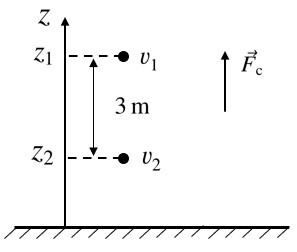
\includegraphics[scale=0.6]{../figs/VN10-PH-33-L-025-3-H1.jpg}
		\end{center}
		Công của lực cản khi vật chuyển động $\SI{3}{\meter}$ là
		\begin{equation*}
			A=F_\text{c}S\cos\alpha=\SI{4}{\newton}\cdot\SI{3}{\meter}\cdot\cos(180^\circ)=\SI{-12}{\joule}.
		\end{equation*}
		
		Cơ năng của vật lúc bắt đầu rơi là
		\begin{equation*}
			W_1=W_\text{đ1}+W_\text{t1}=\dfrac{1}{2}mv_1^2+mgz_1=mgz_1.
		\end{equation*}
		
		Cơ năng của vật sau khi rơi quãng đường $\SI{3}{\meter}$ là
		\begin{equation*}
			W_2=W_\text{đ2}+W_\text{t2}=\dfrac{1}{2}mv_2^2+mgz_2.
		\end{equation*}
		
		Do vật chịu tác dụng thêm lực cản nên cơ năng vật biến đổi. Công của lực cản bằng độ biến thiên cơ năng
		\begin{eqnarray*}
			&&A=W_2-W_1\\
			&\Rightarrow& A = \dfrac{1}{2}mv_2^2+mgz_2 - mgz_1\\
			&\Rightarrow& A= \dfrac{1}{2}mv_2^2+mg(z_2-z_1)\\
			&\Rightarrow& \SI{-12}{\joule} = \dfrac{1}{2}\cdot\SI{1}{\kilogram}\cdot v_2^2 + \cdot\SI{1}{\kilogram}\cdot \SI{10}{\meter/\second^2}\cdot(-\SI{3}{\meter})\\
			&\Rightarrow& v_2 = \SI{6}{\meter/\second}.
		\end{eqnarray*}
		
		\textbf{Đáp án: D.}
		
		\begin{center}
			\textbf{Câu hỏi tương tự}
		\end{center}
		
		Một vật khối lượng $\SI{2}{kg}$ được ném thẳng đứng với vận tốc ban đầu $\SI{20}{m/s}$ xuống đất. Lấy $g=\SI{10}{m/s^2}$. Chọn gốc thế năng tại mặt đất. Bỏ qua lực cản của không khí trong quá trình vật chuyển động.
		\begin{enumerate}[label=\alph*)]
			\item Tính cơ năng của vật lúc ném.
			\item Tìm vận tốc của vật khi chạm đất.
		\end{enumerate}
		
		\textbf{Đáp án:} $\SI{400}{J}$; $\SI{20}{m/s}$.
	}
	\viduii{3}{Một vật có khối lượng $m$ bắt đầu trượt không vận tốc đầu từ đỉnh của một mặt phẳng nghiêng có hệ số ma sát $\mu=0,2$, góc nghiêng $\beta=30^\circ$, $g=\SI{10}{\meter/\second^2}$. Khi vật trượt được quãng đường dài $\SI{10}{\meter}$ trên mặt phẳng nghiêng thì vận tốc của vật là
		\begin{mcq}(4)
			\item $\SI{8}{\meter/\second}$.
			\item $\SI{7}{\meter/\second}$.
			\item $\SI{9}{\meter/\second}$.
			\item $\SI{10}{\meter/\second}$.
		\end{mcq}
	}
	{	\begin{center}
			\textbf{Hướng dẫn giải}
		\end{center}
		
		\textbf{Cách 1:}
		
		\begin{center}
			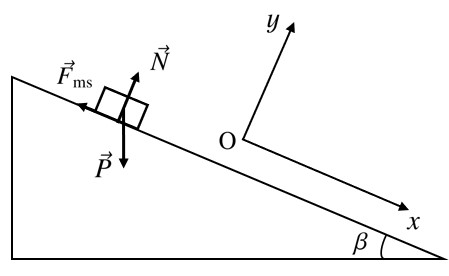
\includegraphics[scale=0.5]{../figs/VN10-PH-33-L-025-3-H2.jpg}
		\end{center}
		
		Chọn O$x$ và O$y$ như hình vẽ.
		
		Các lực tác dụng gồm:
		\begin{itemize}
			\item Lực ma sát $\vec{F}_\text{ms}$;
			\item Trọng lực $\vec{P}$;
			\item Phản lực $\vec{N}$.
		\end{itemize}
		
		Áp dụng định luật II Newton ta được
		\begin{equation*}
			\vec{a}=\dfrac{\vec{P}+\vec{N}+\vec{F}_\text{ms}}{m}.
		\end{equation*}
		
		Chiếu lên O$y$ ta được
		\begin{equation*}
			N = P\cos\beta = mg\cos\beta.
		\end{equation*}
		
		Chiếu lên O$x$ ta được
		\begin{equation*}
			a=\dfrac{P\sin\beta-F_\text{ms}}{m}=\dfrac{mg\sin\beta-\mu mg\cos\beta}{m}=g(\sin\beta-\mu\cos\beta).
		\end{equation*}
		
		Thay số vào ta được
		\begin{equation*}
			a=g(\sin\beta-\mu\cos\beta)=\SI{10}{\meter/\second^2}\cdot (\sin30^\circ-0,2\cdot\cos30^\circ)=\SI{3,27}{m/s^2}.
		\end{equation*}
		
		Theo công thức liên hệ a, v, s trong chuyển động thẳng biến đổi đều ta có
		\begin{equation*}
			v^2-v_0^2=2as\Rightarrow v=\sqrt{v_0^2+2as}=\sqrt{2\cdot \left(\SI{3,27}{m/s^2}\right)\cdot \SI{10}{\meter}}= \SI{8}{\meter/\second}.
		\end{equation*}
		
		Vậy khi vật trượt được quãng đường dài $\SI{10}{\meter}$ trên mặt phẳng nghiêng thì vận tốc của vật là $\SI{8}{\meter/\second}$.
		
		\textbf{Cách 2:}
		
		\begin{center}
			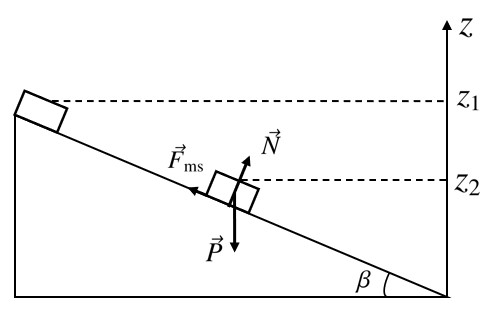
\includegraphics[scale=0.5]{../figs/VN10-PH-33-L-025-3-H3.jpg}
		\end{center}
		
		Chọn mốc thế năng tại vị trí chân mặt phẳng nghiêng.
		
		Các lực tác dụng gồm:
		\begin{itemize}
			\item Lực ma sát $\vec{F}_\text{ms}$;
			\item Trọng lực $\vec{P}$;
			\item Phản lực $\vec{N}$.
		\end{itemize}
		
		Công của lực không thế tác dụng lên vật là
		\begin{eqnarray*}
			A&=&A_\text{ms}+A_N\\
			&=&F_\text{ms}s\cos\alpha+0\\
			&=&\mu N s\cos\alpha\\
			&=&\mu\cdot  mg\cos\beta \cdot s \cdot \cos\alpha
		\end{eqnarray*}
		
		Cơ năng của vật lúc bắt đầu rơi là
		\begin{equation*}
			W_1=W_\text{đ1}+W_\text{t1}=\dfrac{1}{2}mv_1^2+mgz_1=mgz_1.
		\end{equation*}
		
		Cơ năng của vật sau khi rơi quãng đường $\SI{10}{\meter}$ là
		\begin{equation*}
			W_2=W_\text{đ2}+W_\text{t2}=\dfrac{1}{2}mv_2^2+mgz_2
		\end{equation*}
		
		Do vật chịu tác dụng thêm lực cản nên cơ năng vật biến đổi. Công của lực cản bằng độ biến thiên cơ năng
		\begin{eqnarray*}
			A&=&W_2-W_1\\
			\Rightarrow A &=& \dfrac{1}{2}mv_2^2+mgz_2 - mgz_1\\
			\Rightarrow \mu\cdot  mg\cos\beta \cdot s \cdot \cos\alpha &=& \dfrac{1}{2}mv_2^2+mg(z_2 - z_1)\\
			\Rightarrow \mu\cdot  g\cos\beta \cdot s \cdot \cos\alpha &=& \dfrac{1}{2}v_2^2 - g s\sin\beta\\
			\Rightarrow 0,2 \cdot \SI{10}{\meter/\second^2} \cdot \cos 30^\circ \cdot \SI{10}{\meter} \cdot \cos 180^\circ &=& \dfrac{1}{2}\cdot v_2^2 -\SI{10}{\meter/\second^2}\cdot \SI{10}{\meter} \cdot\sin30^\circ\\
			\Rightarrow v_2 &=& \SI{8}{\meter/\second}.
		\end{eqnarray*}
		
		\textbf{Đáp án: A}.
		
		\begin{center}
			\textbf{Câu hỏi tương tự}
		\end{center}
		
		Một viên bi khối lượng $m$ chuyến động ngang không ma sát với vận tốc $\SI{2}{\meter/\second}$ rồi đi lên mặt phẳng nghiêng góc nghiêng $30^\circ$.
		\begin{enumerate}[label=\alph*)]
			\item Tính quãng đường $s$ mà viên bi đi được trên mặt phẳng nghiêng.
			\item Ở độ cao nào thì vận tốc của viên bi giảm còn một nửa?
			\item Khi vật chuyển động được quãng đường là $\SI{0,2}{\meter}$ lên mặt phẳng nghiêng thì vật có vận tốc bao nhiêu?
		\end{enumerate}
		
		\textbf{Đáp án:} $\SI{0.4}{m}$; $\SI{0.15}{m}$; $\xsi{\sqrt 2}{m/s}$.
	}
	
\end{dang}

\begin{dang}{Áp dụng biến thiên cơ năng  để xác định lực tác dụng }
	
	\viduii{3}{
		Một vật khối lượng $\SI{2}{kg}$ được ném thẳng đứng với vận tốc ban đầu $\SI{20}{m/s}$ xuống đất. Lấy $g=\SI{10}{m/s^2}$. Chọn gốc thế năng tại mặt đất. Bỏ qua lực cản của không khí trong quá trình vật chuyển động. Sau khi chạm đất, vật lún sâu $\SI{10}{cm}$ rồi dừng lại. Tính lực cản trung bình của đất.
	}
	{\begin{center}
			\textbf{Hướng dẫn giải}
		\end{center}
		
		Cơ năng của vật tại ví trí ném:
		$$W_1 = W_\text{đ1} + W_\text{t1} = \SI{400}{J}.$$
		
		Cơ năng của vật tại vị trí sâu $\SI{10}{cm}$ dưới đất:
		$$W_2 = 0 + mgz_2 = \SI{-2}{J}.$$
		
		Khi vật dừng lại thì toàn bộ cơ năng chuyển thành công của lực cản của đất:
		$$\Delta W = W_2 - W_1 = \SI{-402}{J}= A_\text{cản} = -F_\text{cản} \cdot \SI{0.1}{m} \Rightarrow F_\text{cản} = \SI{4020}{N}.$$
		
		\begin{center}
			\textbf{Câu hỏi tương tự}
		\end{center}
		
		Một viên bi nhỏ khối lượng $\SI{200}{g}$ được ném thẳng đứng xuống dưới từ điểm O có độ cao $\SI{7}{m}$ so với mặt đất với tốc độ ban đầu $\SI{4}{m/s}$. Bỏ qua sức cản của không khí, lấy $g=\SI{10}{m/s^2}$. Giải bài toán bằng phương pháp năng lượng, chọn gốc thế năng tại mặt đất. Đất mềm, viên bi lún thẳng xuống mặt đất thêm một đoạn $\SI{10}{cm}$. Tính lực cản trung bình của đất tác dụng lên viên bi.
		
		\textbf{Đáp án:} $\SI{158}{N}$.
	}
	\viduii{3}{
		Ném vật khối lượng $\SI{150}{g}$ thẳng đứng lên cao từ mặt đất với vận tốc $\SI{20}{m/s}$. Cho $g=\SI{10}{m/s^2}$. Chọn gốc thế năng tại mặt đất.
		
		Nếu lực cản trung bình của không khí bằng $20\%$ trọng lượng của vật thì độ cao cực đại mà vật đạt được là bao nhiêu?
	}
	{\begin{center}
			\textbf{Hướng dẫn giải}
		\end{center}
		
		Cơ năng:
		$$W_1 = W_\text{đ1} + 0 =\dfrac{1}{2}mv_0^2=\dfrac{1}{2}\cdot\SI{0.15}{\kilogram}\cdot(\SI{20}{\meter/\second})^2= \SI{30}{J}.$$
		
		Lực cản bằng trung bình của không khí tác dụng lên vật  $$F_\text{cản} = 20\%mg = 20\%\cdot\SI{0.15}{\kilogram}\cdot\SI{10}{\meter/\second^2}= \SI{0.3}{\newton}.$$
		
		Công của lực cản tác dụng lên vật từ khi vật ở mặt đất đến khi vật ở độ cao cực đại $h$:
		$$A_\text{cản} = -F_\text{cản} h.$$
		
		Độ biến thiên cơ năng bằng công của lực cản:
		$$\Delta W = W_2 - W_1 = mgh - W_1 = -F_\text{cản} h \Rightarrow h= \SI{16.67}{m}.$$
		
		\begin{center}
			\textbf{Câu hỏi tương tự}
		\end{center}
		
		Một vật có khối lượng $\SI{3}{kg}$ được thả rơi không vận tốc đầu từ độ cao $\SI{4}{m}$ so với mặt đất. Lấy $g=\SI{9.8}{m/s^2}$. Biết ngay trước khi chạm đất vận tốc của vật là $\SI{6}{m/s}$. Hãy tính lực cản trung bình của không khí tác dụng lên vật.
		
		\textbf{Đáp án:} $\SI{15.9}{N}$.
	}
\end{dang}
